\chapter{Modes of Operation}

\section{Introduzione}
Si illustrerà come usare gli algoritmi di crittografia a chiave segreta, DES, IDEA e AES, in applicazioni reali: è stato visto soltanto come usare tali algoritmi per cifrare blocchi di lunghezza prefissata (64 bit per DES e IDEA, 128 bit per AES), come si procede se è necessario cifrare dei messaggi di lunghezza arbitraria/diversa? \newline \newline
Si vedrà inoltre come si generano dei MAC (\textbf{M}essage \textbf{A}uthentication \textbf{C}ode) sfruttando la crittografia a chiave segreta.

\section{Cifrare messaggi di grandi dimensioni}
Come è possibile cifrare messaggi di dimensioni superiori a 64 bit? \newline
Sono state proposte diverse \textbf{modalità operative dei cifrari a blocchi}, cioè ci si è interrogati su come utilizzare i cifrari a blocchi nel caso di messaggi di lunghezza maggiore di quella di un singolo blocco.\newline \newline
Le modalità più conosciute e che verranno descritte di seguito sono:
\begin{itemize}
  \item \textbf{E}lectronic \textbf{C}ode \textbf{B}ook (ECB)
  \item \textbf{C}ipher \textbf{B}lock \textbf{C}haining (CBC)
  \item k-Bit \textbf{C}ipher \textbf{F}eed\textbf{B}ack Mode (CFB)
  \item k-Bit \textbf{O}utput \textbf{F}eed\textbf{B}ack Mode (OFB)
  \item \textbf{C}oun\textbf{T}e\textbf{R} Mode (CTR)
\end{itemize} 
Si noti che nel seguito si farà riferimento a cifrari a blocchi con blocchi di 64 bit (tutte le considerazioni valgono anche nel casi di cifrari con blocchi di dimensione diversa da 64 bit).
\subsection{Electronic Code Book (ECB)}
Questa modalità consiste nel fare la cosa più ovvia, ma corrisponde, in genere, alla soluzione peggiore, cioè:
\begin{itemize}
\item il messaggio viene decomposto in blocchi da 64 bit (inserendo eventualmente dei bit di padding nell'ultimo blocco al fine di riempirlo)
\item ciascun blocco da 64 bit viene cifrato con la chiave segreta
\item ciascun blocco cifrato viene decifrato
\item il messaggio viene ricomposto a partire dai singoli blocchi decifrati
\end{itemize}
Come illustrato nella figure \figurename ~\ref{fig:ECB_enc} e \figurename ~\ref{fig:ECB_dec}
\begin{figure}[htbp]
	\centering%
	\subfigure%
	{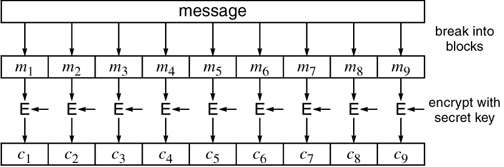
\includegraphics[height=4cm, width=12cm, keepaspectratio]{Immagini/Capitolo3/ECB_enc.png}}
	\caption{Schema di crittografia ECB \label{fig:ECB_enc}} 	
	\subfigure%
	{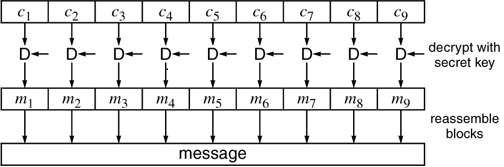
\includegraphics[height=4cm, width=12cm, keepaspectratio]{Immagini/Capitolo3/ECB_dec.png}}
	\caption{Schema di decrittografia ECB \label{fig:ECB_dec}} 
\end{figure}
\subsubsection{Problemi di sicurezza in ECB}
La modalità operativa ECB introduce una serie di problemi non presenti nel cifrario a blocchi: se il messaggio contiene due blocchi di 64 bit identici, allora anche i corrispondenti blocchi cifrati saranno identici e ciò fornisce delle informazioni aggiuntive sul testo in chiaro che un ascoltatore può sfruttare.
\begin{figure}
\centering%
	\subfigure%
	{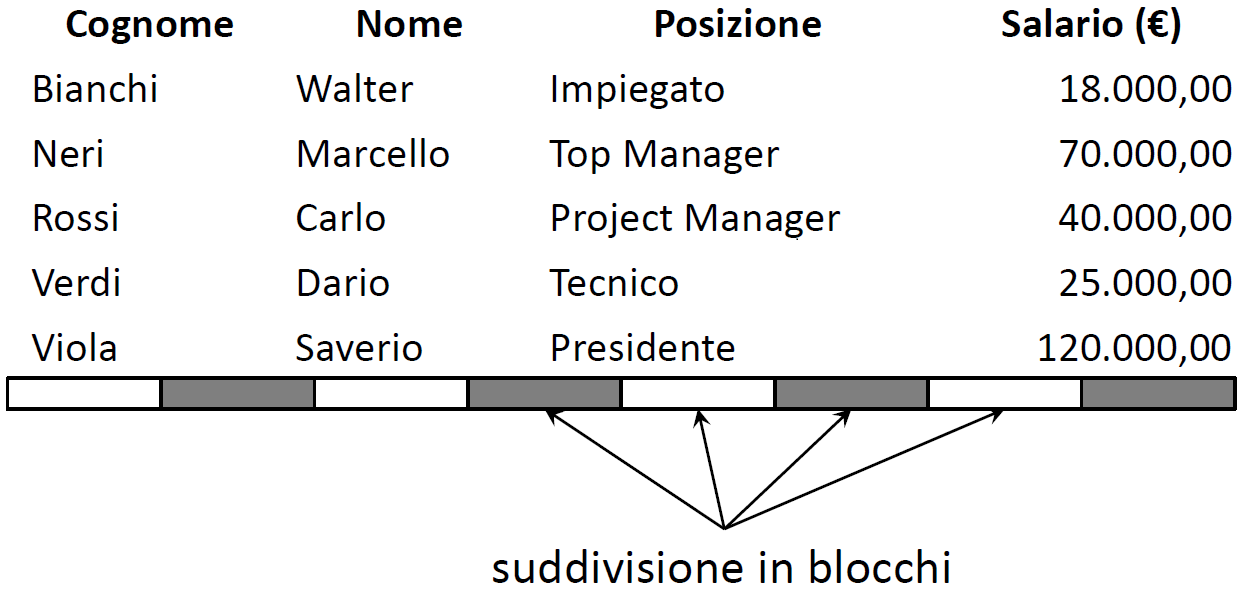
\includegraphics[height=6cm, width=10cm, keepaspectratio]{Immagini/Capitolo3/File_salari.png}}
	\caption{File con i salari, oggetto di attacco \label{fig:File_salari}} 	
\end{figure}
Si consideri ad esempio lo scenario della \figurename ~\ref{fig:File_salari}: supponiamo che l'ascoltatore sappia che il testo in chiaro contiene l'elenco, ordinato alfabeticamente, degli impiegati e dei relativi salari inviato dall'amministrazione all'ufficio paghe, supponiamo inoltre che ogni riga del file sia lunga esattamente 64 byte (8 blocchi da 8 byte) e che i vari blocchi risultino suddivisi in modo tale che alcuni contengono la codifica della cifra decimale più significativa del campo salario (migliaia di dollari/euro). Comparando i testi cifrati, l'ascoltatore, oltre a dedurre quanti dipendenti hanno lo stesso salario, può anche dedurre quanti dipendenti hanno uno stipendio nello stesso range (ordine di 10 euro/dollari); se ci sono complessivamente pochi range salariali, l'ascoltatore può dedurre a quale categoria di dipendente corrisponda un dato blocco cifrato; inoltre, se l'ascoltatore è un impiegato, può sostituire il blocco cifrato di un altro dipendente (un manager) al suo blocco cifrato (dedotto in base all'ordine e alla
numerosità della sua classe salariale).\newline \newline
ECB quindi ha due serie debolezze, legate al fatto che qualcuno, analizzando diversi blocchi cifrati potrebbe:
\begin{itemize}
\item dedurre (inferire) informazioni sfruttando le ripetizioni di alcuni blocchi
\item riarrangiare/modificare i blocchi cifrati a proprio vantaggio
\end{itemize}
Per tali ragioni ECB è raramente usato.
\subsection{Cipher Block Chaining (CBC)}
CBC non presenta i problemi di ECB: a due blocchi in chiaro identici non corrispondono
due blocchi cifrati identici.
\subsubsection{Idea base}
Per comprendere CBC conviene prima considerare il seguente esempio, in riferimento alla \figurename ~\ref{fig:rand_ele_cb_enc} che ne condivide l’idea base:
\begin{itemize}
\item per ogni blocco di testo in chiaro mi viene generato un numero random a 64 bit $r_{i}$
\item $m_{i}$ e $r_{i}$ vengono sommati ($\oplus$ XOR)
\item il risultato viene cifrato con la chiave segreta
\item i blocchi cifrati $c_{i}$ e i numeri random, in chiaro, $r_{i}$ vengono trasmessi
\end{itemize}
E per riottenere il testo in chiaro:
\begin{itemize}
\item vengono decifrati i blocchi $c_{i}$ con la chiave segreta 
\item i blocchi risultanti vengono sommati ($\oplus$ XOR) con i numeri random $r_{i}$
\end{itemize}
\begin{figure}
\centering%
	\subfigure%
	{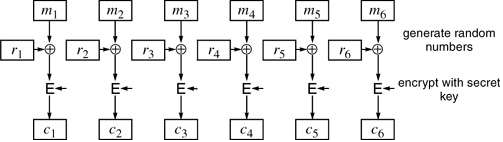
\includegraphics[height=5cm, width=10cm, keepaspectratio]{Immagini/Capitolo3/rand_ele_cb_enc.png}}
	\caption{Randomized Electronic Code Book Encryption\label{fig:rand_ele_cb_enc}} 	
\end{figure}
L'esempio appena visto è molto inefficiente, infatti l'informazione da trasmettere è duplicata perché per ogni blocco va trasmesso il corrispondente numero random. \newline
Un altro problema è che un avversario può riarrangiare i blocchi in modo da ottenere un effetto predittivo sul testo in chiaro, ad esempio:
\begin{itemize}
\item se la coppia $r_{2}|c_{2}$ fosse rimossa il corrispondente blocco in chiaro $m_{2}$ scomparirebbe 
\item se la coppia $r_{2}|c_{2}$ fosse scambiata con la coppia $r_{7}|c_{7} \Rightarrow$ $m_{2}$ e $m_{7}$ risulterebbero scambiati
\item se l’avversario conosce ciascun  $m_{i}$, può modificare  $m_{i}$ in modo predittivo cambiando il corrispondente numero random $r_{i}$
\end{itemize}
\subsubsection{Funzionamento}
CBC genera i “propri” numeri random usando $c_{i}$ come numero random $r_{i+1}$, cioè usa il precedente blocco cifrato come numero random da sommare ($\oplus$ XOR) al blocco di testo in chiaro successivo.\newline
Per evitare che due testi in chiaro inizialmente identici diano luogo a dei blocchi cifrati inizialmente identici CBC genera un singolo numero random, detto vettore di inizializzazione (\textbf{Initialization Vector $IV$}), che viene sommato ($\oplus$ XOR) con il primo blocco di testo in chiaro. \newline
Il risultato viene trasmesso dopo la cifratura a chiave segreta. \newline
La decifratura è semplice essendo l'or-esclusivo un'operazione che coincide con la propria inversa.\newline
Quanto detto, rappresentato nelle figure \figurename ~\ref{fig:CBC_enc} e \figurename ~\ref{fig:CBC_dec}, può essere espresso anche algebricamente:
\begin{itemize}
\item CIFRATURA\newline $c_{1} = E(K, (IV \oplus m_{1}))$\newline $c_{i} = E(K, (c_{i-1} \oplus m_{i})) \forall i > 1$
\item DECIFRATURA\newline $m_{1} = E(K,c_{1})\oplus IV$\newline $m_{i} = E(K,c_{i})\oplus c_{i-1}$
\end{itemize}
\begin{figure}[htbp]
	\centering%
	\subfigure%
	{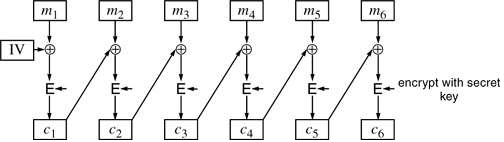
\includegraphics[height=4cm, width=12cm, keepaspectratio]{Immagini/Capitolo3/CBC_enc.png}}
	\caption{Schema di crittografia CBC \label{fig:CBC_enc}} 	
	\subfigure%
	{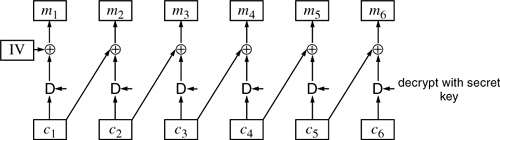
\includegraphics[height=4cm, width=12cm, keepaspectratio]{Immagini/Capitolo3/CBC_dec.png}}
	\caption{Schema di decrittografia CBC \label{fig:CBC_dec}} 
\end{figure}
Si noti che, essendo il costo della somma ($\oplus$ XOR) trascurabile rispetto al costo della cifratura a chiave segreta, la cifratura con CBC ha le stesse prestazioni della cifratura con ECB eccetto il costo delle generazione e trasmissione di $IV$. In molti casi, tuttavia, la sicurezza di CBC non dipende dalla
scelta del vettore di inizializzazione $IV$ (cioè si possono anche porre tutte le cifre di $IV$ pari a 0).\newline \newline
In alcuni casi, tuttavia, l'assenza di $IV$ riduce la sicurezza. Ad esempio, si supponga che il file cifrato contenente i salari dei dipendenti sia trasmesso settimanalmente; in assenza di $IV$, un ascoltatore potrebbe verificare se il testo cifrato differisce da quelle della precedente settimana, e potrebbe determinare la prima persona il cui salario è cambiato. Un altro esempio è quello di un generale che invia
giornalmente delle informazioni segrete dicendo “continue holding your position”; il testo cifrato sarebbe ogni giorno lo stesso, finché il generale decide di cambiare ordine, inviando il messaggio “start bombing”: il testo cifrato cambierebbe immediatamente, allertando il nemico.\newline
Un vettore di inizializzazione scelto randomicamente garantisce che, anche se lo stesso messaggio è inviato ripetutamente, il corrispondente testo cifrato risulta ogni volta differente, e previene attacchi all'algoritmo di cifratura di tipo testo in chiaro selezionato anche quando un avversario può fornire del testo in chiaro al CBC.
\subsubsection{CBC minaccia 1 – Modifica dei blocchi cifrati}
L’uso di CBC non elimina il problema che qualcuno possa modificare il messaggio in transito, semplicemente cambia la natura della minaccia: un avversario non può più vedere ripetizioni di blocchi cifrati, e non può più copiare/spostare blocchi cifrati (ad esempio per scambiare il salario di due dipendenti) ma può ancora modificare il testo cifrato in modo predittivo. \newline
Cosa potrebbe succedere se modificasse un blocco di testo cifrato, ad esempio $c_{n}$?\newline
Da $m_{n+1} = E(K,c_{n+1})\oplus c_{n}$ si evince che una modifica di $c_{n}$ può avere un effetto prevedibile su $m_{n+1}$ (ad esempio, cambiando il terzo bit di $c_{n}$ cambia il terzo bit di $m_{n+1}$);
chiaramente essendo anche $m_{n} = E(K,c_{n})\oplus c_{n-1}$,  l'avversario non può prevedere quale possa essere il nuovo valore di $m_{n}$, molto probabilmente la modifica di $c_{n}$ corrompe completamente il blocco in chiaro $m_{n}$.\newline
Vediamo a tal proposito l'esempio seguente, illustrato in \figurename ~\ref{fig:modifica_blk_cifrati}:
\begin{figure}[htbp]
	\centering%
	\subfigure%
	{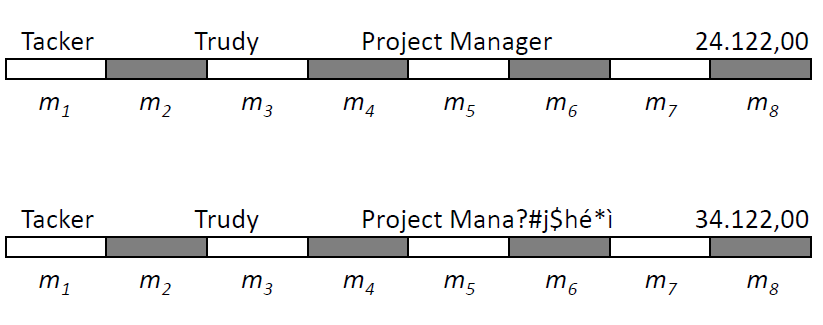
\includegraphics[height=4cm, width=12cm, keepaspectratio]{Immagini/Capitolo3/modifica_blk_cifrati.png}}
	\caption{Modifica dei blocchi cifrati \label{fig:modifica_blk_cifrati}}	
\end{figure}
\newline Supponiamo che un avversario (Trudy) sappia che una data sequenza di blocchi cifrati, del file
dei salari, corrispondano alla riga contenente i suoi dati personali; se Trudy vuole aumentare il suo salario di 10K, e se sa che l'ultimo byte di $m_{7}$ corrisponde alle decine di migliaia nella codifica decimale (00000010), per darsi 10K in più deve semplicemente cambiare il bit meno significativo di $c_{6}$; da $m_{7} = D(K, c_{7}) \oplus c_{6}$ tuttavia, Trudy non sarà più in grado di predire cosa apparirà nella voce “Posizione”, infatti, da $m_{6} = D(K, c_{6}) \oplus c_{5}$, si vede che è impraticabile
prevedere l'effetto della modifica di $c_{6}$ su $m_{6}$. Se il file decifrato fosse letto da una persona umana, questa potrebbe insospettirsi della presenza di simboli strani nel campo “Posizione”, se invece il file decifrato viene elaborato da un programma l'attacco potrebbe non essere rilevato.\newline \newline
Ricapitolando: Trudy è stato in grado di modificare un blocco in modo predittivo con l'effetto collaterale di modificare il blocco precedente senza poter prevedere il risultato finale.
\subsubsection{CBC minaccia 2 – Riarrangiamento blocchi cifrati}
Con riferimento alla \figurename ~\ref{fig:riarrangiamento_blk_cifrati}, si supponga che Trudy conosca il testo in chiaro e, il corrispondente testo cifrato di qualche messaggio, cioè $m_{1}$, $m_{2}$, ..., $m_{n}$ e $IV$, $c_{1}$, $c_{2}$, ..., $c_{n}$; in questo modo Trudy conosce automaticamente anche il blocco decifrato di ciascun $c_{i}$, da $D(K, c_{1}) = c_{i-1} \oplus m_{i}$.
\begin{figure}[htbp]
	\centering%
	\subfigure%
	{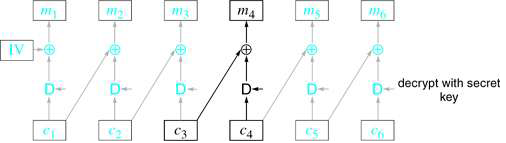
\includegraphics[height=3cm, width=12cm, keepaspectratio]{Immagini/Capitolo3/riarrangiamento_blk_cifrati.png}}
	\caption{Riarrangiamento dei blocchi cifrati \label{fig:riarrangiamento_blk_cifrati}}	
\end{figure}
Da queste informazioni, Trudy può considerare ciascun $c_{i}$ come un "building block" e costruire un flusso cifrato usando ogni combinazione di $c_{i}$ ed essere in grado di calcolare quale sarà il corrispondente testo in chiaro. \newline \newline
Per capire a cosa potrebbe servire questo tipo di attacco si tenga presente che uno dei modi di combattere la minaccia di modifica di blocchi cifrati è includere un \textbf{CRC} (\textbf{C}yclic \textbf{R}edundancy \textbf{C}heck) al testo in chiaro prima di cifrarlo con un CBC, perciò se Trudy modifica qualche blocco cifrato, il CRC consentirà ad un computer di rilevare prontamente l'alterazione del messaggio (e.g. se si fosse scelto un CRC a 32 bit ci sarebbe una possibilità su $2^32$ che il CRC coincida con quello corretto); supponiamo che a Trudy non interessi quale possa essere il nuovo messaggio di testo in chiaro (che potrebbe essere completamente indecifrabile), ma interessi solamente che il nuovo messaggio manomesso sia accettato dal computer ricevente sapendo che viene eseguito un controllo di tipo CRC, Trudy può provare a costruire molti flussi cifrati combinando in modi diversi i blocchi $c_{1}$, $c_{2}$, ..., $c_{n}$ e può calcolare il risultante testo in chiaro per ciascuno di essi, per poi testare se il testo in chiaro risultante ha un CRC corretto (mediamente serviranno $2^31$ tentativi).\newline 
Che male potrebbe fare Trudy modificando un messaggio, senza controllarne il contenuto, in modo
tale che sia accettato dal computer ricevente? Forse Trudy è soltanto maliziosa, e vuole distruggere
alcuni dati che vengono caricati attraverso la rete, ma in realtà, c'è un modo sottile di controllare, seppur in misura ridotta, il contenuto del messaggio modificato: supponiamo che Trudy sposti blocchi contigui, ad esempio, se $c_{n}$ e $c_{n+1}$ vengono spostati in qualche altro posto, allora il blocco originale $m_{n+1}$ apparirà in un'altra posizione; se $m_{n+1}$ contiene il salario del presidente, Trudy
potrebbe scambiare i blocchi in modo da cambiarlo con il suo, ma poi dovrà modificare molto probabilmente gran parte del messaggio restante per garantire che il CRC risulti invariato.\newline \newline
Per prevenire attacchi di questo tipo, basati sul riarrangiamento dei blocchi cifrati e tali da preservare il CRC originario, potrebbe essere usato un CRC a 64 bit: ciò è sicuramente sufficiente se l'attacco al CRC, nell'ambito di un CBC, è di tipo a forza bruta. \newline
Per chi progetta protocolli crittografici sicuri, una modalità di cifratura ad un singolo step che protegga sia la confidenzialità che l'autenticità di un messaggio è stata per molti anni una sorta di "Sacro Graal" da ricercare!
\subsection{Output FeedBack Mode (OFB)}
L’OFB è un cifrario a flusso: la cifratura consiste nel sommare ($\oplus$ XOR) il messaggio con il keystream (o one-time pad) generato da OFB stesso. Supponiamo che il keystream sia ottenuto generando singoli blocchi di 64 bit alla volta; un possibile modo per generarlo è il seguente:
\begin{itemize}
\item viene generato un numero random $IV$ (Initialization Vector) di 64 bit
\item il primo blocco del keystream coincide con $IV$: $b_{0} = IV$
\item i blocchi seguenti $b_{i}$ si ottengono cifrando $b_{i-1}$ con la chiave segreta: $b_{i} = E(K,b_{i-1})$
\end{itemize}
Il one-time pad (keystream) risultante è dato dalla sequenza $OTP = OTP(K, IV) = b_{0}|b_{1}|b_{2}|…|b_{i}|b_{i+1}|…$.
La cifratura con OFB (\figurename ~\ref{fig:OFB_enc}) consiste nel sommare ($\oplus$ XOR) il messaggio $m$ con OTP, se $m$ ha lunghezza $l_{m}$ bit si considereranno soltanto $l_{m}$ bit di OTP.
\begin{figure}[htbp]
	\centering%
	\subfigure%
	{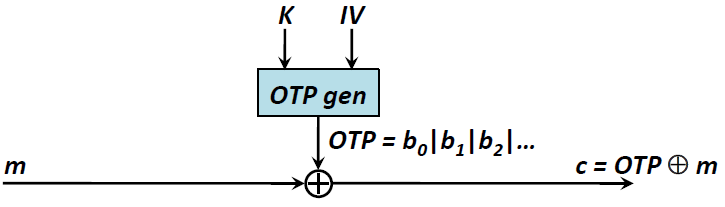
\includegraphics[height=4cm, width=12cm, keepaspectratio]{Immagini/Capitolo3/OFB_enc.png}}
	\caption{Schema di crittografia OFB \label{fig:OFB_enc}} 	
\end{figure}
Il risultato della cifratura $c = OTP \oplus m$ viene trasmesso insieme a $IV$ (la lunghezza $l_{c}$ di c coincide con $l_{m}$).\newline
In decifratura (\figurename ~\ref{fig:OFB_dec}) il destinatario riceve $IV$ e conoscendo $K$ calcola lo stesso onetime pad $OTP = OTP(K, IV)$  il messaggio $m$ si ottiene sommando ($\oplus$ XOR) il flusso cifrato $c$ con $l_{c}$ bit di OTP.
\begin{figure}[htbp]
	\centering%
	\subfigure%
	{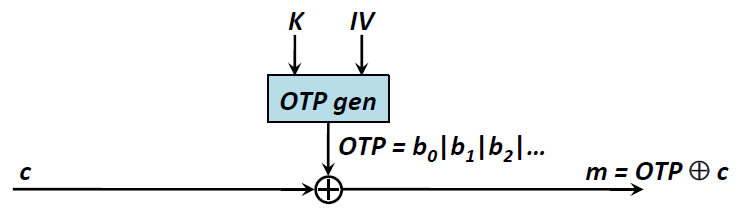
\includegraphics[height=4cm, width=12cm, keepaspectratio]{Immagini/Capitolo3/OFB_dec.png}}
	\caption{Schema di decrittografia OFB \label{fig:OFB_dec}} 	
\end{figure}
\subsubsection{Vantaggi e svantaggi di OFB}
OFB presenta i seguenti vantaggi:
\begin{itemize}
\item visto che il one-time pad OTP può essere generato in anticipo, prima che sia noto il messaggio m da cifrare, una volta ottenuto m è necessario soltanto effettuare la somma ($\oplus$ XOR) con il one-time pad (lo XOR è eseguibile in modo estremamente veloce)
\item se qualche bit del testo cifrato dovesse corrompersi, soltanto i corrispondenti bit del testo in chiaro sarebbero corrotti, diversamente dalla modalità CBC, dove se $c_{n}$ fosse corrotto allora $m_{n}$ sarebbe completamente corrotto e $m_{n+1}$ sarebbe corrotto in corrispondenza dei medesimi bit di $c_{n}$
\item un messaggio m può arrivare a pezzi di lunghezza arbitraria, e, ogni volta che arriva un pezzo, il corrispondente testo cifrato può essere immediatamente trasmesso; in CBC invece, se il messaggio arriva un byte alla volta, per la cifratura è comunque necessario attendere che un blocco di 64 bit (o un multiplo intero di 8 byte) sia completo (ciò può comportare l'attesa di altri 7 byte o l'aggiunta di bit di riempimento, cosa che aumenta la quantità di dati da trasmettere)
\end{itemize}
OTP ha però anche il seguente svantaggio:
\begin{itemize}
\item se un avversario conoscesse il testo in chiaro m e quello cifrato c, potrebbe modificare il testo in
chiaro a piacimento semplicemente sommando il testo cifrato con il testo in chiaro noto, e sommando il risultato con un qualsiasi messaggio $m'$ che desidera sostituire ad m; cioè l'avversario dovrebbe modificare il testo cifrato come $c' = c \oplus m \oplus m'$ e verificare che decifrando $c'$ anziché $c$ si ottiene $m'$ anziché $m$.
\end{itemize}
\subsection{k-bit Output FeedBack Mode (k-OFB)}
In generale la modalità OFB consente di generare flussi di "pezzi" da $k$ bit (quanto visto prima corrisponde al caso in cui $k$ = 64 bit).
La modalità k-bit OFB funziona nel seguente modo (si descriverà la versione data in [DES81]) con riferimento alla \figurename ~\ref{fig:k-bit_OFB}:
\begin{figure}[htbp]
	\centering%
	\subfigure%
	{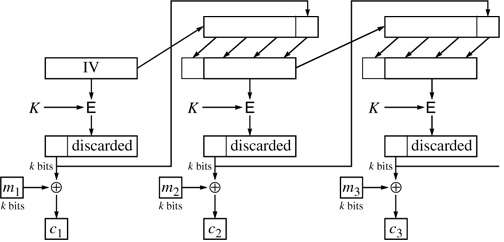
\includegraphics[height=4cm, width=12cm, keepaspectratio]{Immagini/Capitolo3/k-bit_OFB.png}}
	\caption{k-bit OFB \label{fig:k-bit_OFB}} 	
\end{figure}
\begin{itemize}
\item l'input $I_{0}$ al modulo di cifratura DES è inizializzato a $IV$, cioè $I_{0}=IV$: se $IV$ ha meno di 64 bit, vengono inseriti degli 0 di riempimento a sinistra (cifre più significative)
\item il primo pezzo $b_{0}$ di OTP si ottiene selezionando $k$ bit dall’output $O_{0} = E(K, I_{0})$ di DES (una quantità a 64 bit); da un punto di vista crittografico non ha importanza come siano scelti tali bit da $O_{0}$; [DES81] specifica che devono essere i $k$ bit più significativi
\item l’i-esimo pezzo $b_{i}$ si ottiene selezionando i $k$ bit più significativi dell'output $O_{i} = E(K, I_{i})$ di DES, ove l'input $I_{i}$ è stato ottenuto da $I_{i-1}$ eseguendo una traslazione a sinistra di $k$ bit, e un inserimento di $b_{i-1}$ nei $k$ bit meno significativi di $I_{1}$ ($k$ bit più a destra)
\end{itemize}
\subsection{Cipher FeedBack Mode (CFB)}
La modalità CFB è molto simile a OFB, con riferimento alla \figurename ~\ref{fig:k-bit_CFB}:
\begin{figure}[htbp]
	\centering%
	\subfigure%
	{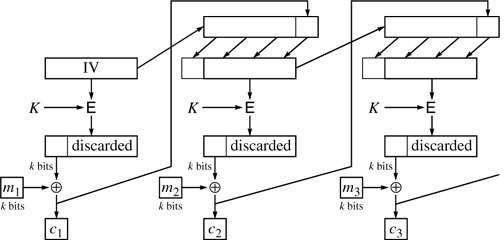
\includegraphics[height=4cm, width=12cm, keepaspectratio]{Immagini/Capitolo3/k-bit_CFB.png}}
	\caption{k-bit CFB \label{fig:k-bit_CFB}} 	
\end{figure}
\begin{itemize}
\item viene prodotto un one-time pad generando, uno alla volta, singoli pezzi di $k$ bit
\item il one-time pad viene sommato ($\oplus$ XOR) con pezzi di $k$ bit del messaggio
\end{itemize}
Si noti che in OFB i $k$ bit meno significativi dell'input $I_{i}$ del modulo di cifratura DES sono i $k$ bit di $b_{i-1}$ (sono parte dell'output $O_{i-1}$ della cifratura DES del blocco precedente; invece, in CFB i $k$ bit di $I_{i}$ sono i $k$ bit di testo cifrato del blocco precedente, cioè i $k$ bit di $c_{i-1}$ (in CFB il one-time pad non può essere generato prima che il messaggio e noto, a differenza di OFB), nella modalità a k-bit è ragionevole assegnare a $k$ un valore diverso da 64 bit (una scelta sensata è $k$ = 8 bit).
\subsubsection{Vantaggi e svantaggi  di CFB}
CBF presenta i seguenti vantaggi:
\begin{itemize}
\item Con OFB o CBC, se si ha una perdita di caratteri in trasmissione (testo cifrato), i.e. se nel flusso cifrato $c_{1}, c_{2}, c_{3}, ... , c_{n}, ...$ si perde il carattere $c_{k}$, allora a destinazione si ottiene la sequenza $c_{1}, c_{2}, c_{3}, ... , c_{k'}, ... , c_{n-1'}$ ove $c_{k'} = c_{k+1}, c_{k+1'} = c_{k+2}, ... , c_{k+i'} = c_{k+i+1}$; oppure, con OFB o CBC, se extra caratteri sono aggiunti al flusso cifrato, i.e. se nel flusso cifrato$c_{1}, c_{2}, c_{3}, ... , c_{n}, ...$ si aggiunge il carattere $c*$ dopo di $c_{k-1}$, allora a destinazione si ottiene la sequenza $c_{1}, c_{2}, c_{3}, ... , c_{k'}, ... , c_{n+1'}$ ove $c_{k'} = c*, c_{k+1'} = c_{k}, ... , c_{k+i'} = c_{k+i-1}$. Quindi l'intera parte restante della trasmissione risulta indecifrabile poiché $m_{i’} = c_{i’} \oplus b_{i}$ e $b_{i} = b_{i}(K, IV)$ cioè bi non dipende dalla sequenza cifrata. Invece, con 8-bit CFB, si ha un effetto risincronizzante: se un byte ci è perso in trasmissione allora corrispondente testo in chiaro mi è perso, e i successivi 8 byte $m_{i+1}, …, m_{i+8}$ risulteranno indecifrabili, ma dal byte $m_{i+9}$ in poi il testo in chiaro sarà corretto, questo perché $b_{i} = b_{i}(K, c_{i-1})$, cioè $b_{i}$ è derivato dalla sequenza di caratteri cifrati. Discorsi analoghi valgono nel caso dell'aggiunta di un byte al flusso cifrato.
\item i messaggi cifrati con CFB offrono più protezione di CBC e di OFB rispetto ad eventuali manomissioni; infatti, nel caso di 8-bit CFB un avversario può modificare ogni singolo byte in modo predittivo, ma con l'effetto collaterale di non poter prevedere/controllare i successivi 8 byte discorsi simili valgono per 64-bit CFB.
\item a differenza di CBC, non sono possibili attacchi basati sul riarrangiamento di blocchi; tuttavia intere sezioni del messaggio possono essere riarrangiate rendendo indecifrabili le parti corrispondenti ai "punti di giuntura".
\end{itemize}
CBF ha anche i seguenti svantaggi:
\begin{itemize}
\item 8-bit CFB ha lo svantaggio che ogni byte di input richiede un'operazione DES. Inizialmente CFB fu concepito per essere utilizzato con un numero arbitrario $k$ di bit per "pezzo", con $k$ minore della dimensione di un blocco completo (64 bit per DES); nella pratica tuttavia $k$ è pari a 1 byte oppure coincide con la dimensione piena (full-block) dei blocchi del modulo di cifratura. Quando utilizzato in modalità full-block le prestazioni di CFB sono comparabili a quelle di ECB, CBC, e OFB.
\item come OFB consente di cifrare ed inviare ciascun byte del messaggio non appena è noto tuttavia, a differenza di OFB non è in grado di anticipare il calcolo del one-time pad in fine, è in grado di rilevare delle alterazioni meglio di OFB, ma non bene quanto CBC.
\end{itemize}
\subsection{CounTeR Mode (CTR)}
CTR (\figurename ~\ref{fig:CTR}) è simile a OFB perché un one-time pad viene generato e sommato ($\oplus$ XOR) con i dati; tuttavia differisce da OFB perché non concatena ciascun blocco di one-time-pad con il precedente, ma incrementa $IV$ e poi cifra quanto ottenuto per ottenere il prossimo blocco di one-time pad. 
\begin{figure}[htbp]
	\centering%
	\subfigure%
	{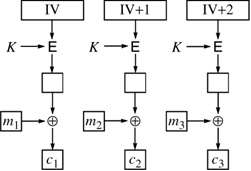
\includegraphics[height=4cm, width=12cm, keepaspectratio]{Immagini/Capitolo3/CTR.png}}
	\caption{CTR \label{fig:CTR}} 	
\end{figure}
\subsection{Vantaggi e svantaggi di CTR}
Il vantaggio principale di CTR è che, come OFB, il one-time pad può essere pre-calcolato, e la cifratura consiste in un semplice XOR; inoltre, come in CBC, la decifratura di un messaggio può iniziare da un qualunque blocco (non e obbligata ad iniziare dal primo blocco). Per questo CRT è l'ideale in applicazioni che richiedono la cifratura di file/memorie ad accesso casuale (sottoinsiemi di dati prelevati ed ordine non prevedibili).\newline \newline
Come in OFB (e in tutti i cifrari a flusso), nella modalità CTR si ha una perdita di sicurezza se messaggi diversi sono cifrati con la stessa coppia $\langle K, IV \rangle$, poichè un avversario potrebbe ottenere la somma ($\oplus$ XOR) dei testi in chiaro se somma ($\oplus$ XOR) due testi cifrati ottenuti con la stessa coppia $\langle K, IV \rangle$.

\section{Generare message authentication code(MAC)}
Un sistema di cifratura a chiave segreta può essere usato per generare un MAC cioè un checksum cifrato: \textbf{MAC} sta per \textbf{M}essage \textbf{A}uthentication \textbf{C}ode. \\
Un sinonimo di MAC è \textbf{MIC} (\textbf{M}essage \textbf{I}ntegrity \textbf{C}ode) e, anche se il termine MAC è più popolare; nella \textbf{PEM} (\textbf{P}rivacy \textbf{E}nhanced \textbf{M}ail) viene usato il termine MIC.\\
\\
Le modalità operative CBC, CFB, OFB, e CTR offrono una buona protezione della confidenzialità, i.e. un messaggio intercettato è difficilmente decifrabile, ma non offrono una buona protezione dell'integrità/autenticità di un messaggio, i.e. non proteggono da ascoltatori che lo modificano in modo non rilevabile.\\
Nel seguito useremo i termini integrità e autenticità in modo intercambiabile visto che se il messaggio é integro allora non è stato modificato dal momento in cui è stato generato, i.e. il messaggio è autentico.
\subsection{Residuo CBC}
Un modo standard per assicurare l'autenticità di un messaggio $m$ (cioè per proteggersi da modifiche di $m$ non rilevabili) è, in riferimento alla \figurename ~\ref{fig:residuo_CBC} :
\begin{itemize}
\item calcolare il CBC di $m$
\item inviare soltanto l'ultimo blocco cifrato (64 bit) e il messaggio $m$ in chiaro; l'ultimo blocco cifrato è detto \textbf{residuo CBC}.
\end{itemize}
\begin{figure}[htbp]
	\centering%
	\subfigure%
	{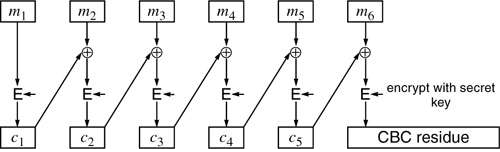
\includegraphics[height=4cm, width=12cm, keepaspectratio]{Immagini/Capitolo3/residuo_CBC.png}}
	\caption{Residuo CBC \label{fig:residuo_CBC}} 	
\end{figure}
Il calcolo del residuo CBC richiede la conoscenza della chiave segreta $K$, quindi se un avversario modifica $m$ in $m’$ allora $res_{CBC}(m’)$ sarà diverso da $res_{CBC}(m)$ (c'è solo 1 possibilità su $2^64$ che siano uguali) perchè l'avversario non è in grado di calcolare $res_{CBC}(m’)$ senza conoscere la chiave segreta $K$. \\
Il destinatario del messaggio calcola il residuo del messaggio in chiaro ricevuto, e verifica che sia uguale al residuo ricevuto; se i residui coincidono deduce che (con elevata probabilità) il residuo ricevuto è stato calcolato da qualcuno che conosce la chiave segreta, i.e. il mittente è autentico.\\
\\
In molte applicazioni non è necessario proteggere la confidenzialità, ma solo l'autenticità; in questi casi si può trasmettere il testo in chiaro più il residuo. Tuttavia, è assai frequente la necessità di
proteggere contemporaneamente confidenzialità e autenticità: se il messaggio $m$ è un singolo blocco, ciò può ottenersi con una semplice cifratura a chiave segreta. Nel caso di un messaggio multi blocco qual è la
trasformazione equivalente?
\subsection{Assicurare confidenzialità e autenticità}
Dato un messaggio $m$:
\begin{itemize}
\item per assicurare la \textbf{confidenzialità} di $m$ basta cifrarlo in modalità CBC
\item per assicurare l'\textbf{autenticità} di $m$ basta inviare $res_{CBC}(m)$ più $m$ in chiaro
\end{itemize}
Allora a prima vista la soluzione riportata in \figurename ~\ref{fig:residuo_CBC_1} sembrerebbe assicurare confidenzialità e autenticità:
\begin{figure}[htbp]
	\centering%
	\subfigure%
	{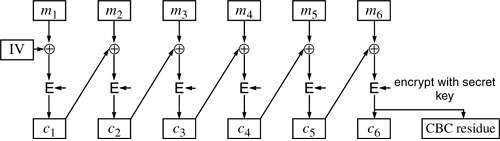
\includegraphics[height=4cm, width=12cm, keepaspectratio]{Immagini/Capitolo3/residuo_CBC_1.png}}
	\caption{Assicurare confidenzialità e autenticità: soluzione 1 \label{fig:residuo_CBC_1}} 	
\end{figure}
In realtà tale soluzione è chiaramente errata, infatti consiste nell'inviare il messaggio cifrato nella modalità CBC ($E_{CBC}(K, IV, m)$) ripetendo soltanto l'ultimo blocco cifrato ($res_{CBC}(m)$); così chiunque voglia alterare il messaggio deve solo modificare uno o più blocchi cifrati con CBC e inviare il nuovo messaggio ripetendo due volte l'ultimo blocco cifrato. \\
Quindi inviare il residuo CBC in aggiunta al messaggio cifrato con CBC non aumenta la sicurezza. \\ 
Si noti infatti che per autenticità (integrità) intendiamo che un calcolatore è in grado di rilevare automaticamente se il messaggio è stato alterato. Usando CBC da solo, allora, non è possibile rilevare in
modo automatico eventuali modifiche di un messaggio, poiché ogni stringa di bit, comunque venga generata, viene decifrata in "qualcosa", e gli ultimi 64 bit di quella stringa sono il suo residuo CBC corretto; in questo modo chiunque intercetti il testo cifrato può modificarlo, e un computer a destinazione decifrerà il risultato, che potrebbe essere assolutamente privo di senso, senza essere consapevole che quanto ottenuto è di fatto spazzatura. \\
Un utente umano si renderebbe conto che il testo cifrato è stato alterato, a meno che la modifica non sia stata eseguita da un avversario in modo "pulito", ma un computer non è in grado di farlo se non si
aggiunge un controllo di integrità.\\ \\
Un'alternativa potrebbe essere calcolare il residuo CBC del messaggio $res_{CBC}(m)$, allegarlo al testo in chiaro $m$, e cifrare con CBC la concatenazione $m|res_{CBC}(m)$ (\figurename ~\ref{fig:residuo_CBC_2})
\begin{figure}[htbp]
	\centering%
	\subfigure%
	{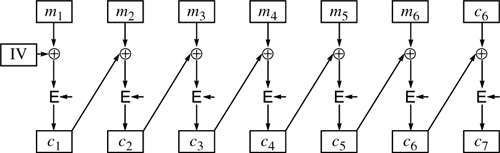
\includegraphics[height=4cm, width=12cm, keepaspectratio]{Immagini/Capitolo3/residuo_CBC_2.png}}
	\caption{Assicurare confidenzialità e autenticità: soluzione 2 \label{fig:residuo_CBC_2}} 	
\end{figure}
In realtà neanche questa soluzione funziona, infatti: $c_{7} = res_{CBC}(m) = E(K, c_{6} \oplus c_{6}) = E(K, 000 … 0)$, cioè il residuo CBC è una stringa ottenuta cifrando con la chiave segreta una stringa di 64 bit a 0, quindi il residuo CBC non dipende da $m$ e non può offrire alcune protezione di integrità.\\ \\
Come altra alternativa, supponiamo di calcolare un checksum non crittografico $CRC(m)$ (ad esempio, un CRC) del messaggio $m$ e di appenderlo alla fine di $m$, e di cifrare con CBC il tutto: $m| CRC(m)$, secondo lo schema in \figurename ~\ref{fig:residuo_CBC_3}
\begin{figure}[htbp]
	\centering%
	\subfigure%
	{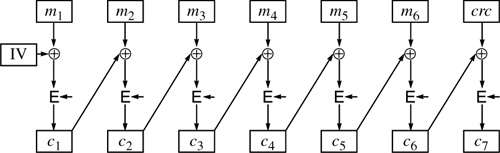
\includegraphics[height=4cm, width=12cm, keepaspectratio]{Immagini/Capitolo3/residuo_CBC_3.png}}
	\caption{Assicurare confidenzialità e autenticità: soluzione 3 \label{fig:residuo_CBC_3}} 	
\end{figure}
Questa soluzione "quasi" funziona: è vulnerabile ad attacchi molto sottili se il CRC è corto, d'altro canto checksum non crittografici più lunghi sono "sospetti". \\ 
\subsubsection{Soluzione sicura}
Viene considerata una soluzione sicura quella che riesce a proteggere la confidenzialità di un messaggio $m$ cifrandolo con CBC, e l'integrità di $m$ con un residuo CBC, a patto che vengano usate due chiavi distinte, $K$ e $K'$:
\begin{itemize}
\item confidenzialità: $E_{CBC}(K, IV, m)$
\item integrità: $res_{CBC}(K', IV, m)$
\end{itemize}
Chiaramente ciò comporta una notevole perdita di efficienza, infatti il costo computazionale è duplicato rispetto al
costo della sola cifratura CBC. \\
Sono state proposte tecniche più rapide, ma generalmente presentano sempre dei "sottili difetti" crittografici (se tali difetti siano seri o meno dipende dal tipo di applicazione e dall'intelligenza dell'avversario); alcune di queste tecniche sono:
\begin{itemize}
\item \textbf{CBC con un Checksum Crittografico Debole}: Visto che l'uso di checksum non crittografici in CBC risulta poco sicuro, e che checksum crittografici di qualità sono computazionalmente dispendiosi, è stato proposto di usare checksum crittografici "deboli". Complessivamente dovrebbe essere una soluzione sicura, infatti lo sforzo computazionale per violare il checksum debole va moltiplicato per le limitazioni derivanti dal fatto che è usato
in una cifratura CBC. Sebbene non ci sono ragioni per sostenere che tale schema sia insicuro, CBC con checksum crittografici deboli non ha riscosso successo (si consideri che Kerberos IV usa un checksum crittografico debole per la protezione d'integrità fuori da uno schema di cifratura e sembra che non sia mai stato violato!)
\item \textbf{Cifratura CBC e Residuo CBC con Chiavi Correlate}: anziché usare due chiavi completamente indipendenti per la cifratura CBC e per il calcolo del residuo, un trucco usato in Kerberos V è impiegare una versione modificata della chiave in una delle due operazioni. Cambiare un singolo bit dovrebbe essere sufficiente, ma Kerberos invece somma ($\oplus$ XOR) la chiave con la costante a 64 bit $F0F0F0F0F0F0F0F0_{16}$; tale soluzione preserva la parità della chiave e non trasforma mai una chiave non-debole in una chiave debole. Il fatto di avere una chiave matematicamente correlata all'altra (in alternativa alla scelta di due numeri random come chiavi) non introduce particolari debolezze, ma non introduce neanche particolari vantaggi (in generale, distribuire una coppia di chiavi non è più difficile di distribuirne solo una, e il fatto che due chiavi siano matematicamente correlate non riduce il carico computazionale, l'unico vantaggio nel derivare una chiave dall'altra lo si ha quando si dispone di un sistema/servizio per la distribuzioni di chiavi singole che non è estendibile al caso di coppie di chiavi).
\item \textbf{CBC con Hash Crittografico}: un altro approccio è concatenare un messaggio m con il suo un hash
crittografico $h(m)$, tipicamente 128 bit, e cifrare con CBC il tutto, $m|h(m)$. Tale soluzione è probabilmente sicura, sebbene non sia stata adeguatamente studiata, visto che gli schemi moderni usano hash cifrati con chiavi richiede due fasi crittografiche (come nel caso della cifratura CBC più il residuo CBC con chiavi distinte), ma è più efficiente se la funzione di hash è più veloce dell'algoritmo di cifratura 
\item \textbf{Offset Codebook Mode (OCB)}: OCB è uno dei molti modi che permette di ottenere cifratura e protezione di integrità effettuando soltanto una singola fase di cifratura. OCB e altre tecniche simili sono molto recenti per
avere un supporto di studi e test, spesso sono gravate da licenze/patenti, ma sembra molto probabile che una o più di
queste tecniche diventi alla fine il modo standard per ottenere protezione di integrità e di confidenzialità.
\end{itemize}

\section{Cifratura multipla DES}
\subsection{Cifratura multipla EDE o 3DES}
In generale, ogni schema di cifratura può essere reso più sicuro ricorrendo alla cifratura multipla.
Nel caso di DES, è universalmente ritenuta sicura la procedura nota come EDE.
\textbf{E}ncrypt-\textbf{D}ecrypt-\textbf{E}ncrypt (o 3DES, \textbf{triplo DES}):
\begin{itemize}
\item $c = E(K_{1},D(K_{2},E(K_{1},m))) = (E_{1} o D_{2} o E_{1})(m)$
\item $m = D(K_{1},E(K_{2},D(K_{1},c))) = (D_{1} o E_{2} o D_{1})(c)$
\end{itemize}
La cifratura multipla EDE è di fatto un meccanismo per incrementare la lunghezza della chiave DES. Sebbene sia stata introdotta per arrivare ad uno standard sicuro basato su DES, in linea di principio è applicabile anche ad altri schemi
di cifratura, ed esempio ad IDEA, ma è più importante nel caso di DES poiché la chiave DES è notoriamente considerata troppo corta.\\ \\
Si è visto che uno schema di crittografia presenta sempre due funzioni, note come cifratura e decifratura; tali funzioni sono l'una l'inversa dell'altra, i.e.: ciascuna prende in input un blocco di dati $m$, e restituisce il corrispondente blocco offuscato $c$ tale che, applicando a $c$ l'altra funzione si ottiene $m$. Ha quindi senso applicare la "funzione di decifratura" $D(K, m)$ al testo in chiaro $m$ per cifrarlo e poi applicare la "funzione di cifratura" $E(K, D(K, m))$ per decifrare quanto ottenuto riottenendo il testo in chiaro $m$; ma in definitiva ha poco senso chiamare $E(K, m)$ "funzione di cifratura", e $D(K, m)$ "funzione di decifratura", poiché i ruoli di tali funzioni sono interscambiabili. Conviene chiamarle semplicemente \textbf{funzione $E()$} e \textbf{funzione $D()$} (tuttavia, spesso si continuerà a chiamarle funzione di cifratura e funzione di decifratura).\\ \\
Realizzare una cifratura multipla non è banale, specie se si desidera anche ottenere un cifrario a flusso a partire da un cifrario a blocchi. \\
Il metodo standard per usare EDE è il seguente: vengono usate due chiavi (e non tre), $K_{1}$ e $K_{2}$ e ogni blocco di testo in chiaro $m_{i}$ è sottoposto prima ad $E_{1}()$ (cioè viene eseguito $E(K_{1}, m)$), poi a $D_{2}()$ (cioè viene eseguito $D(K_{2}, E(K_{1}, m))$) e in fine ancora ad $E_{1}()$ (cioè viene eseguito $E(K_{1}, D(K_{2},
E(K_{1}, m)))$).\\
Quanto ottenuto è di fatto un nuovo schema di cifratura a chiave segreta (\figurename ~\ref{fig:EDE}): un blocco di 64 bit in input è mappato in un altro blocco di 64 bit in output; il processo è invertibile se si conoscono le chiavi, altrimenti è di fatto impraticabile risalire dall'output all'input.
\begin{figure}[htbp]
	\centering%
	\subfigure%
	{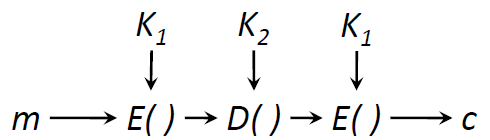
\includegraphics[height=2cm, width=10cm, keepaspectratio]{Immagini/Capitolo3/EDE.png}}
	\caption{Cifratura EDE o 3DES \label{fig:EDE}} 	
\end{figure}
La decifratura EDE è semplicemente il processo inverso (\figurename ~\ref{fig:DED}):
\begin{figure}[htbp]
	\centering%
	\subfigure%
	{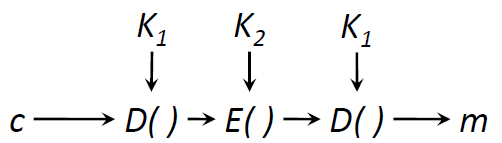
\includegraphics[height=2cm, width=10cm, keepaspectratio]{Immagini/Capitolo3/DED.png}}
	\caption{Decifratura EDE \label{fig:DED}} 	
\end{figure}
\subsection{EDE con CBC Outside/Inside}
Per ottenere un cifrario a flusso (i.e. la corrispondente modalità operativa di flusso) a partire dal cifrario a blocchi EDE, viene usata la modalità operativa \textbf{CBC outside}, i.e. le tre funzioni $E_{1}()-D_{2}()-E_{1}()$ vengono applicate a ciascun blocco, ma il concatenamento CBC viene eseguito soltanto una volta (\figurename ~\ref{fig:EDE_CBC_Out}).\\ 
\begin{figure}[htbp]
	\centering%
	\subfigure%
	{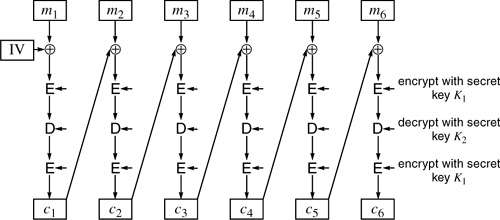
\includegraphics[height=4cm, width=12cm, keepaspectratio]{Immagini/Capitolo3/EDE_CBC_Out.png}}
	\caption{EDE con CBC Outside \label{fig:EDE_CBC_Out}} 	
\end{figure}
Il cifrario a flusso è ottenibile anche con un concatenamento \textbf{CBC inside}, i.e. si considerano una cascata di tre concatenamenti CBC (semplificando alcuni passaggi): prima utilizzando $CBC-E_{1}()$, poi utilizzando $CBC-D_{2}()$ e infine utilizzando ancora $CBC-E_{1}()$ (\figurename ~\ref{fig:EDE_CBC_In}).
\begin{figure}[htbp]
	\centering%
	\subfigure%
	{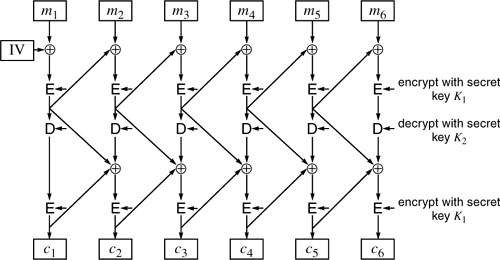
\includegraphics[height=4cm, width=12cm, keepaspectratio]{Immagini/Capitolo3/EDE_CBC_In.png}}
	\caption{EDE con CBC Inside \label{fig:EDE_CBC_In}} 	
\end{figure}
\subsubsection{CBC Outside vs Inside}
Il 3DES comunemente usato nelle applicazioni esegue un concatenamento CBC esterno: ad ogni blocco viene applicata la cifratura tripla e il concatenamento CBC viene fatto una sola volta sui blocchi cifrati. L'alternativa sarebbe cifrare completamente il messaggio con $K_{1}$ e CBC, poi decifrare il risultato con $K_{2}$ e CBC, e in fine cifrare di nuovo quanto ottenuto con $K_{1}$ (CBC interno).\\
Quali sono le implicazioni di queste scelte?\\ \\
Si è visto che con CBC è possibile fare una modifica predittiva sul testo in chiaro $m_{n}$ (ad esempio invertire il bit $x$) invertendo il bit $x$ nel blocco cifrato $c_{n-1}$; ciò comporta però l'effetto collaterale di modificare
in modo imprevedibile il blocco $m_{n-1}$, la possibilità di sfruttare questa debolezza dipende dal tipo di applicazione.\\ \\
Con CBC esterno, un avversario può ancora sferrare questo tipo di attacco (il fatto che la cifratura è fatta con un triplo DES è del tutto ininfluente): un avversario che inverte il bit $x$ di un blocco cifrato $c_{n-1}$ modificherà completamente e in modo imprevedibile il blocco di testo in chiaro $m_{n-1}$ (il blocco di testo in chiaro $m_{n}$ avrà il bit $x$ invertito e tutti i blocchi di testo in chiaro diversi da $m_{n-1}$ e $m_{n}$ saranno invariati.\\ \\
Con CBC interno, una modifica ad un blocco cifrato $c_{n}$ altera in modo imprevedibile tutti i blocchi di testo in
chiaro dal blocco $m_{n}$ fino alla fine del messaggio. Per questo CBC interno è più sicuro di CBC esterno, e forse
dovrebbe essere la scelta migliore; tuttavia, in alcuni casi è preferibile che la modifica di un blocco cifrato non si propaghi completamente nel resto del messaggio, i.e. sarebbe preferibile che lo schema di cifratura sia autosincronizzante (dopo un piccolo numero di blocchi corrotti, il testo in chiaro inizierà ad essere nuovamente decifrato correttamente). \\
Un altro vantaggio di CBC interno riguarda l'efficienza: triplicando l'uso di hardware e pipeline per le cifrature si può ottenere complessivamente una velocità pari a quella di una singola cifratura (con CBC esterno ciò non è possibile).\\
CBC interno presenta comunque delle sottili vulnerabilità se un avversario può esaminare l'output e fornire del testo in chiaro scelto e $IV$.\\ \\
Una ragione per la quale CBC esterno è più usato nonostante i suoi svantaggi è che la cifratura EDE può considerarsi a tutti gli effetti un nuovo schema di cifratura (a chiave segreta) a blocchi che usa una chiave di 112 bit, perciò può essere utilizzata con ciascun metodo di concatenamento (OFB, ECB, CFB, CTR e CBC).
